\documentclass[12pt]{article}
    
        \usepackage[utf8x]{inputenc}
        \usepackage[T1]{fontenc}
        \usepackage{lmodern}
        \usepackage{marvosym}
        \usepackage{graphicx}
        \usepackage{hyperref}
        \usepackage{float}
        \usepackage{natbib}
        \usepackage{amsmath}
        \usepackage{cite}
        \hypersetup{
            colorlinks=true,
            linkcolor=blue,
            filecolor=magenta,      
            urlcolor=blue,
        }
        
        \pagestyle{empty}
        
        \usepackage[scale=0.75]{geometry}
        \setlength{\parindent}{0pt}
        \addtolength{\parskip}{6pt}
        \begin{document}
    
    
        \begin{minipage}[c]{1.0 \textwidth}
            \begin{center}
                \Large{\textbf{Seperate Earthqukaes from Nuclear explosions}}\\[0.5em]
                Sabber Ahamed\\
                \today
            \end{center}
        \end{minipage}\\[2em]
        
        \section{Project Overview}
            
        The Comprehensive Nuclear-Test-Ban Treaty (CTBT) is a multinational treaty aim to ban all nuclear activities including explosions, for both civilian and military purposes.  More than 180 countries have agreed and signed the agreement.  But, forty-four countries that have the existing nuclear capabilities must sign and approve the deal for it to have the force of law. Several recognized monitoring systems are used to control the potential violations of the treaty. Seismic wave observation is one of them and is considered the most reliable method for verifying an underground explosion. Seismic stations typically detect as many as 800,000 earthquakes worldwide. Compare to this number, explosions especially the number of nuclear explosions are very-low. Seismologists use several observations such as polarization, p-wave, S-wave and surface wave, depth of the events, etc. to distinguish explosions signal from earthquakes. All the process are complicated and requires the integration of physical and statistical techniques and human interpretations. Not always all the reviews are right. For example, recent quake from North Korea with magnitude 3.0 was first identified as nuclear explosions both by China and South Korea, but the detailed study of the seismic waves later confirmed that the quake was indeed a natural earthquake~\citep{telegraphNatural2017}. Machine learning approach has been adopted to minimizing error in discriminating mine seismic events from mine blasts~\citep{dong2016discrimination}. In this project, my primary goal is to develop an improved machine learning model that can separate natural earthquake from nuclear explosions using raw seismogram.
        
        \section{Problem Statement}
        I plan to use supervised learning techniques toward the final solution. The primary goal is to develop a machine learning model that can distinguish natural earthquakes from nuclear explosions. Since there are only two types of data (earthquakes and nuclear explosions), the model would be binary classification problem. I plan to use support vector machine (SVM) because the preliminary studies show that SVM outperforms the other supervised algorithms such as random forest, Xgboost, LightGBM, etc. More details of SVM is described in algorithoms and techniques sections. The justification for using SVM is discussed in benchmark section. Performance of the model will be evaluated by accuracy, recall, F-1 and ROC-AUC scores based on the predicted and actual values of the test dataset.
    
    
        \section{Metrics}
        In this project, I will use the following evaluation metrics:  
        
        \begin{enumerate}
    
            \item \textbf{Confusion matrix:} The confusion matrix is a convenient presentation of a model performance have multiple classes. The matrix presents predictions on the x-axis and accuracy outcomes on the y-axis. The table helps us understanding the model performance showing positive and negative classes prediction status. 
            
            \item \textbf{Accuracy:} Accuracy measures the proportion of the number of correct predictions of the entire data sets. The metric is the most common and straightforward evaluation metric for classification problems. However, this parameter would not give us very detail information about the model performance and therefore,  can be misused. As a result, I also use the other evaluation metrics listed below.
    
            \item \textbf{precision:} The metric measures the proportion of the positive-class among the total number of positive predictions. Precision would help us to analyze how the model is doing in each category.
            
            \item \textbf{Recall:} Recall on the other hand measures the proportion of the positive-class among the total number of positive-class. The recall is the ideal metric to judge the model performance on positive-class (Nuclear explosions).
            
            \item \textbf{F-1 Score:} This metric combines merely precision and recall just taking the harmonic mean of them. F-score would be my auxiliary evaluation metric after precision and recall because it explicitly represents recall and precision under the hood.
    
            \item \textbf{ROC-AUC score:} Area under ROC Curve (or AUC for short) is a performance metric that represents the model’s ability to discriminate between positive and negative classes. An area of 1.0 represents a model that made all predictions perfectly. Since the project is a binary classification problem, this score would help to evaluate the model performance. I would also use this metric as secondary as F-1 Score. 
        
        \end{enumerate}
        
        % Other than recall and F1-score, the confusion matrix is interesting since it provides information on the performance of the model on a set of test data for which the actual values are known. The results will be evaluated based on the predicted and the real values of the testing dataset.
    
        \section{Analysis}
        \subsection{Data Exploration}
        I will use the facilities of Incorporated Research Institutions for Seismology (IRIS) Data Services, and specifically, the IRIS Data Management Center, to access waveforms, related metadata, and derived products used in this study. IRIS Data Services are funded through the Seismological Facilities for the Advancement of Geoscience and EarthScope (SAGE) Proposal of the National Science Foundation under Cooperative Agreement EAR-1261681. Table-\ref{tab:events_list} shows the events I use for this study. 
    
        \begin{table}[!ht]
            \caption{Seismic events used for this study}
            \vspace{0.5em}
            \label{tab:events_list}
            \centering
            \begin{tabular}{ l c c c c}
            \hline
             Event Origin & Date & Magnitude & Seismograms & Event type \\
             \hline 
              
             % Earthquakes
             Banda Sea & Oct. 24, 2017 & 6.7 & 3382 & Earthquake\\
             Sumatra, Indonesia & Dec. 26, 2004 & 9.0 & 1193 &  Earthquake \\
             Myanmar India border & Mar. 12, 2010 & 5.5 & 3021 & Earthquake \\
             Ryukyu islands & Aug. 15, 1017 & 4.9 & 2644 &  Earthquake \\
             Chiapas Mexico & Sep. 08, 2017 & 8.1  & 2722 &  Earthquake \\
             \hline
             Total & & & 12962 &\\
             \hline
             \hline
             % Nuclear explosions
             India & May. 11, 1998 & 5.2 & 459 & Nuclear explosions \\
             Pakistan & May. 28, 1998 & 4.8 & 470 & Nuclear explosions \\
             Pakistan & May. 30, 1998 & 4.6 & 398 & Nuclear explosions \\
             North Korea & Feb. 12, 2013 & 5.1  & 3763 & Nuclear explosions \\
             North Korea & Jan. 06, 2016 & 5.1  & 2640 & Nuclear explosions \\
             North Korea & Sep. 03, 2017 & 6.3  & 2804 & Nuclear explosions \\
             \hline
             Total & & & 10534 &\\
             \hline
            \end{tabular}
        \end{table}
    
        \begin{table}[ht]
            \caption{Features for the model}
            \vspace{0.5em}
            \label{tab:feature_list}
            % \centering
            \begin{tabular}{l p{0.55\textwidth} c }
                \hline
                Feature Name & Description & Features \\
                \hline
                MFCCs & Mel-frequency cepstral coefficients. & 40\\
                Chorma-stft & Chromagram representing the 12 distinct chromas. & 12 \\
                Amplitude & Maximum and mean amplitude of a waveform & 2\\
                Spectral centroid & Measures the 'center of mass' of a waveform. & 1\\
                Statistical parameters & Moment, variation, skew, variance, auto-corelation, kurtosis. & 6 \\
                \hline
                Total Number of features & & 61 \\
                \hline
            \end{tabular}
        \end{table}
    
    
        \begin{figure}[!htb]
            \begin{center}
            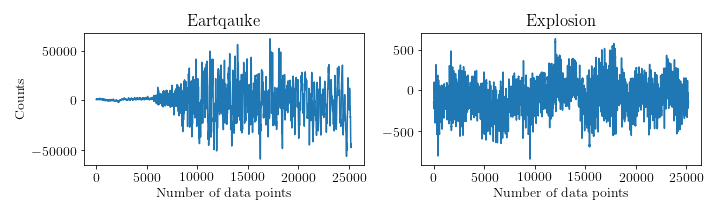
\includegraphics[scale=0.6]{figures/raw_seismograms.png}
            \end{center}
            \caption{The illustration shows the raw east-west componet of earthquake and explosions seismogram recorded at station 'MLAC'.  The earthquake occured in Sumatra, Indonesia in 20014.  The right pannel shows the seismogram due to underground nuclear explosion in India Pakistan border in 1998.}
            \label{fig:raw_seismograms}
        \end{figure}
    
        Each seismogram is 21 minutes long and starts 1 minute before \textit{P}-wave arrival and ends 20 minutes after \textit{P}-wave arrival. Fig.~\ref{fig:raw_seismograms} shows the raw east-west component of seismogram of an earthquake and a nuclear explosion. Characteristics signal features that will be extracted using \texttt{Librosa}~\citep{mcfee2015librosa}- a python package for music and audio analysis. To improve the performance of the model, the number of features may vary in the final solution. I use 20$\%$ f the entire data for testing the model performance.
        
        \subsection{Exploratory Vizualization}
        
        \begin{figure}[!htb]
            \begin{center}
            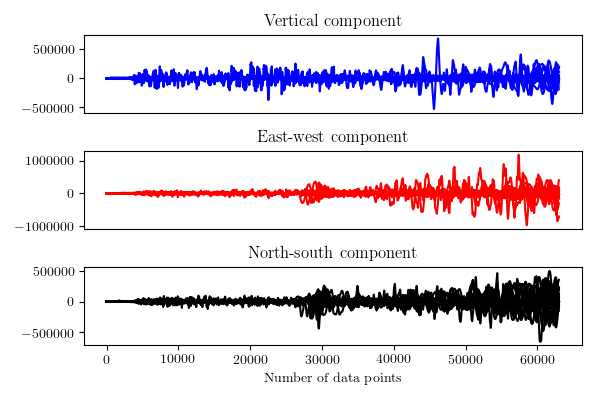
\includegraphics[scale=0.8]{figures/stacked_earthquakes.png}
            \end{center}
            \caption{The illustration shows the 200 stacked seismograms of different earthquakes. Since the seismograms are raw and unprocessed, $x$ and $y$ label do not show usual label like velocity and time respectively. The illustration shows an interesting pattern among the seismograms. For example around 3000 data points $S$-wave arrival is distinctive followed by surface waves after 4000 data points in east-west and north-south component. On the other hand, P-wave arrival is distinctive in vertical component.}
            \label{fig:stacked_earthquakes.png}
        \end{figure}
    
        Fig.~\ref{fig:stacked_earthquakes.png} and~\ref{fig:stacked_explosions.png} shows the stacked seismograms of earthquakes and explosions. Stacked earthquake seismograms show an exciting pattern. For example around 3000 data points $S$-wave arrival is distinctive followed by surface waves after 4000 data points in east-west and north-south component. P-wave arrival time, on the other hand, is characteristic in vertical-component. The explosions seismograms do not show any interesting pattern like earthquake seismograms. The pattern shown by the natural earthquake seismograms would be the key for machine learning models.
    
        \begin{figure}[H]
            \begin{center}
            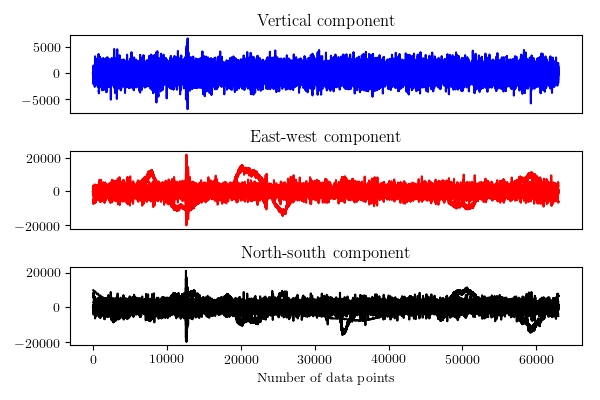
\includegraphics[scale=0.8]{figures/stacked_explosions.png}
            \end{center}
            \caption{The illustration shows the 200 stacked seismograms of different underground nuclear explosions. Sicne seismograms are raw and unprocessed x and y label do not show usual label like velocity and time. The seismograms do not show any interesting pattern like earthquake seismograms.}
            \label{fig:stacked_explosions.png}
        \end{figure}
        
        \subsection{Algorithoms and Techniques}
    
        \subsubsection{Algorithom}
        In this project, I use support vector machine (SVM) algorithm~\citep{cortes1995support} to discriminate natural earthquakes from nuclear explosions.  The algorithm uses kernel trick to transform the data and based on these transformations; it finds an optimal boundary (line or hyperplane) between the possible outputs. An SVM model is a representation of the data points in space, creating a line or hyperplane so that the examples are divided by reasonably. SVM then maps new instances into that same space and predicts a class based on which side of the hyperplane they fall. Vladimir N. Vapnik and Alexey Ya. Chervonenkis in 1963 first present the idea of SVM algorithm. Since then, SVMs have been used successfully in different real-world problems such as text categorization, image classification, protein classification, Cancer analysis, handwritten character recognition, etc.
        
        \subsubsection{Tuning parameters}
        
        In this project I use most widely used the library for implementing machine learning algorithms in python is $\texttt{scikit-learns}$~\citep{scikit-learn}. The following parameters are the significant parameters  need to be tuned to get best model performance :
        
        \begin{enumerate}
            \item C:  It is the regularization parameter, C, of the error term.
            \item kernel: It specifies the kernel type of the algorithm. It can be ‘linear,' ‘poly,' ‘rbf,' ‘sigmoid,' ‘precomputed.
            \item Gamma: Kernel coefficient for ‘rbf,' ‘poly,' and ‘sigmoid.' If gamma is ‘auto,' then 1/n-features will be used instead.
        \end{enumerate}
        
        % \subsubsection{Finding best parameters}
        To find the best parameters I will perform an exhaustive search over specified parameter values using \texttt{scikit-sklearn} implemented $\texttt{GridSearchCV}$. 
        
        \subsection{Benchmark}
        Table-\ref{tab:model_benchmark} listed five supervised algorithms used to create the benchmark. In these benchmarks, I used sklearn~\citep{scikit-learn} default parameters. It is pretty obvious that the support vector machine (SVM) performs better than all other algorithms. Therefore, I use SVM as the final model while its scores set the benchmark for further improvement.
        
        \begin{table}[!ht]
            \caption{Model performance in five algorithoms}
            \vspace{0.5em}
            \label{tab:model_benchmark}
            \centering
            \begin{tabular}{l c c c c}
                \hline
                Algorithom & Accuracy & ROC-AUC & Avg. F1-score & Avg. recall \\
                \hline
                Random Forest & 0.64 & 0.64 & 0.64 & 0.65 \\
                Xgboost & 0.61 & 0.60 & 0.61 & 0.61 \\
                LightGBM & 0.48 & 0.41 & 0.42 & 0.48 \\
                Gaussian Naive Bayes & 0.50 & 0.63 & 0.41 & 0.50 \\
                Support Vector machine & 0.77 & 0.76 & 0.78 & 0.78 \\
                \hline
            \end{tabular}
        \end{table}
        
        \section{Methodology}
        \subsection{Data processing}
        In this project data processing is two-step processing (1) First removing bad seismograms and then apply z-score in each seismogram and (2) Process features extracted from seismogram. The following subsection has the details of these two steps.
        
        \subsubsection{Seismogram processing}
    
        One of the primary objectives of this project is to use raw seismograms to see if the unprocessed seismogram can providing us the information we want. Processing techniques vary person to person and purpose to purpose. In this project, I standardize the seismograms removing the mean from each seismogram so that they are centered around and zero. Other than the standardization I did not use any additional processing necessary for a seismic signal such as instrument corrections and filtering.
    
        \subsubsection{Extracted feature processing}
        Standardization of a dataset is a standard requirement for many machine learning estimators: they might misbehave if the individual feature does not more or less look like standard normally distributed data. After I extract all the features from seismograms, I standardize the features by subtracting the mean and divide by standard deviation.
        
        \subsection{Implementation}
        The implementation process is split into two main steps:
        \begin{enumerate}
            \item Training and 
            \item Measuring the performance
        \end{enumerate}
    
        \begin{figure}[!htb]
            \begin{center}
            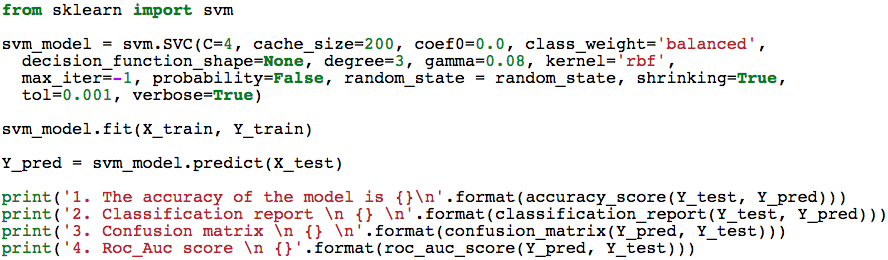
\includegraphics[scale=0.5]{figures/svm_code_snippet.png}
            \end{center}
            \caption{The illustration shows a portion of code snippet implemented to create the model using SVM. The first part of the snippet is importing SVM module from \texttt{scikit-sklearn}. SVM model is created using the parameters obtained by another interesting \texttt{scikit-sklearn} implemented module \texttt{GridSearchCV}. Finally I print out the model performance using evaluation metrics.}
            \label{fig:svm_code_snippet}
        \end{figure}
    
         
        4000 preprocessed training datasets were used to train the model. I use Jupyter-notebook for its interactive and friendly environment. In this project, I use \texttt{scikit-sklearn} implemented API for \texttt{LIBSVM} - an integrated software for support vector classification~\citep{scholkopf2000new}. Each time I get results from the model trained with new sets of parameters I use the evaluation metrics to measure the model$'$s performance. Fig.~\ref{fig:svm_code_snippet} shows a code snippet of the SVM model.
        
    
        \subsection{Refinement}
    
        After I train and build the model, I improved the model accuracy while tuning parameters feature engineering, seismogram processing. The followings are the steps I followed to refine the model performance :
    
        \begin{enumerate}
            \item \textbf{Step 0 Benchmark:} At this initial step I used five of supervised algorithms to find out the best one that gives the highest model performance. I have found Support vector machine is the one provides best model performances regarding accuracy, Recall, F-1, and ROC score. The total number of features is 61 while the accuracy is 77$\%$.
    
            \item \textbf{Step 1 Grid search:} After I select SVM as the final algorithm, I use \texttt{scikit-sklearn} \texttt{GridSearchCV} module to find best C and gamma parameters. After an exhaustive search for many hours, the best C and gamma are 4.0 and 0.08. The total number of features is 61 while the accuracy is 84.5$\%$. 
    
            \item \textbf{Step 2 Feature manipulation:} At this stage, I manipulate some features. I have tried adding some extra features like amplitude of the signal, Mel coefficients, etc. But the did not improve while removing the feature $moment$ increases the accuracy and recall little bit and becomes 85.8$\%$ and 82$\%$ respectively.
    
            \item \textbf{Step 3 Feature manipulation:} At this stage, I add ten more features which improve the model accuracy and positive recall to 87.85$\%$ and 86$\%$ respectively.
    
        \end{enumerate}
    
        \section{Results}
        \subsection{Model evaluation and validation}
        
        \begin{table}[!htb]
            \caption{Confusion matrix based on 4692 testing data} \vspace{0.5em}
            \label{tab:confusion_matrix}
            \centering
            \begin{tabular}{l c c}
            \hline
             & Negative & Positive\\
            \hline
            Natural Earthquakes & True Negative(TN) = 2317 & False negative(FN) = 301 \\
            Nuclear Explosions & False positive(FP) = 269 & True Positive(TP) = 1805 \\
            \hline
            \end{tabular}
        \end{table}
    
        I use 4692 testing data to estimate generalization error of the model created by support vector machine. The table~\ref{tab:confusion_matrix} shows the confusion matrix contains information about actual and predicted classifications. In this project the positive class is \textit{nuclear explosion} and \textit{natural earthquake} is the negative class. The SVM classifier accurately predicts 2322 as earthquakes out of 2594 earthquakes datapoints and 1760  datasets as nuclear explosions out of 2098 explosions data points while rest of the data are misclassified.
        
        %  RF classification result
        \begin{table}[!htb]
            \caption{Classification results based on 4692 testing data} \vspace{0.5em}
            \label{tab:classification_report}
            \centering
            \begin{tabular}{l c c c c}
                \hline
                Class & Precision & Recall & F-1 score & support\\
                \hline
                Natural Earthquke & 0.89 & 0.90 & 0.89 & 2586 \\
                Nuclear explosion & 0.87 & 0.86 & 0.86 & 2106\\
                Average/Total & 0.88 & 0.88 & 0.88 &4692\\[1ex]
                \hline
            \end{tabular}
        \end{table}
    
        Table~\ref{tab:classification_report} shows the classification report using three evaluation metrics. The overall testing accuracy of the model is about $88\%$.  Accuracy measures the proportion of correctly classified classes out of total test datasets. In addition to accuracy, we also consider precision, recall, and f-1 scores. Precision measures how many datasets are correctly classified as true positive among the true and false positive combined.  Whereas, the recall measures the proportion of the correctly identified true positive instances among the total positive datasets. The F-1 score is the harmonic mean of recall and precision.

        % \subsection{Robustness of the Model}
        % I have tested the robustness of the model with an earthquake occurred on May 25, 2009, in Chile-Bolivia border region, the magnitude is 4.1, and a nuclear explosion happened in North Korea on same day May 25 of 2009 with almost same magnitude 4.7. All the new data are processed separately. The purpose of choosing the same day and nearly the same magnitude is to see if the model can perform better in this unknown data sets.
        
        %         \begin{table}[!htb]
        %             \caption{Classification results based on 23460 unknown data} \vspace{0.5em}
        %             \label{tab:robust_classification_report}
        %             \centering
        %             \begin{tabular}{l c c c c}
        %                 \hline
        %                 Class & Precision & Recall & F-1 score & support\\
        %                 \hline
        %                 Natural Earthquke & 0.97 & 0.97 & 0.97 & 12962 \\
        %                 Nuclear explosion & 0.96 & 0.96 & 0.96 & 10498\\
        %                 Average/Total & 0.97 & 0.97 & 0.97 &23460\\[1ex]
        %                 \hline
        %             \end{tabular}
        %         \end{table}
        
        % Interestingly the model outperforms the testing performance. The new accuracy and ROC-AUC score are 96.85$\%$ and9 96.81$\%$ The table~\ref{tab:robust_classification_report} show the detail evaluation report on the classification. I am amazed to see the robustness of the model which motivates me to publish this result and model as a paper as soon as possible. I believe the model will help both the scientific and political community to track recent North Korea's nuclear activity.

        
        \subsection{Justification}
        The final ROC-AUC score of the model is 87.76$\%$ which is 10.22$\%$ more than that of the benchmark. To judge the model performance on positive-class (nuclear explosions), we need to look at the misclassification. In the benchmark, the model misclassified 30.11$\%$ atomic explosions while the final results misclassified 16.67$\%$. The model also successfully identifies the recent nuclear explosion in North Korea~(Fig.~\ref{fig:predicted_seismogram}), which is a great performance. In summary, the current model is helpful to discriminate the signals recorded only in the USA, however, to solve the bigger problem we need more data hence powerful hardware with multiple CPUs or GPUs.
    
        \section{Conclusion}
        \subsection{Free-Form Vizualization}

        \begin{figure}[H]
            \begin{center}
            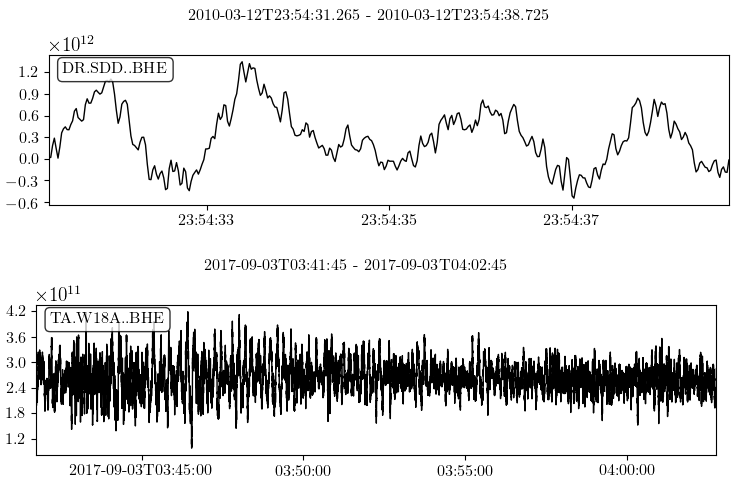
\includegraphics[scale=0.5]{figures/predicted_seismogram.png}
            \end{center}
            \caption{The illustration shows a correctly predicted earthquake and nuclear explosions. The earthquake occurred in Myanmar India border in 2004 and recorded in station 'SDD,' USA. The underground explosion occurred recently in 2017 in North Korea and recorded by 'W18A' station of TA network in the USA.}
            \label{fig:predicted_seismogram}
        \end{figure}

        \subsection{Reflection}
        The processed used for this project can be listed as follows :
        \begin{enumerate}
            \item Select earthquake and nuclear explosions events.
            \item A request has been submitted to IRIS to get the data.
            \item Processes the seismograms and remove bad and noisy ones.
            \item Extract features from each seismogram
            \item Create a benchmark for the classifier and find the best algorithm.
            \item The classifier was trained using trained data.
            \item \texttt{GridSearchCV} was used to find the best parameters to improve the model performance.
            \item Manipulate the features to increase the model performance. 
        \end{enumerate}
    
        I found step four is the most difficult since I had to familiarize the sound signal processing library \texttt{Librosa} and several techniques. Another problematic but exciting part of the project was to manipulate the features (step eight). I’m also happy and grateful for getting to use open source libraries like \texttt{scikit-sklearn}, \texttt{Librosa}, \texttt{Jupyter-notebook}, \texttt{numpy, scipy} as I believe open-sourcing scientific works helps our researchers to discover essential things for humankind.
    
        \subsection{Improvement}
        Distinctive and useful features are required to achieve the optimal model performance. Using raw seismograms was one of the most challenging. If I had used processed and three components seismogram together to determine features,  the model performance would be improved definitely. However, my motivation was to use raw seismograms to see if they are capable of discriminating between earthquakes and nuclear explosions. I believe feature selections are the key to improve the model performance.
        
        \bibliographystyle{plain}
        \bibliography{report_referneces}
        
        \end{document}